
\documentclass[border=8pt, multi, tikz]{standalone} 
\usepackage{import}
\subimport{../layers/}{init}
\usetikzlibrary{positioning}
\usetikzlibrary{3d} %for including external image 
\usepackage{amsbsy}
\usepackage{amsmath}

\def\ConvColor{rgb:yellow,5;red,2.5;white,5}
\def\ConvReluColor{rgb:yellow,5;red,5;white,5}
\def\PoolColor{rgb:red,1;black,0.3}
\def\UnpoolColor{rgb:magenta,5;black,20}
\def\ResBlocksColor{rgb:blue,5;black,30}
\def\StrideOneColor{rgb:blue,5;red,2.5;white,5}
\def\StrideTwoColor{rgb:red,1;black,0.3}
\def\TransConvColor{rgb:blue,2;green,1;black,0.3}
\def\AffineColor{rgb:yellow,5;red,2.5;white,5}
\def\FcColor{rgb:blue,5;red,2.5;white,5}
\def\FcReluColor{rgb:blue,5;red,5;white,4}
\def\SoftmaxColor{rgb:magenta,5;black,7}   
\def\SumColor{rgb:blue,5;green,15}
\def\ConcatColor{rgb:blue,5;red,2.5;white,5}

\newcommand{\copymidarrow}{\tikz \draw[-Stealth,line width=0.8mm,draw={rgb:blue,4;red,1;green,1;black,3}] (-0.3,0) -- ++(0.3,0);}

\begin{document}
\begin{tikzpicture}
\tikzstyle{connection}=[ultra thick,every node/.style={sloped,allow upside down},draw=\edgecolor,opacity=0.7]
\tikzstyle{copyconnection}=[ultra thick,every node/.style={sloped,allow upside down},draw={rgb:blue,4;red,1;green,1;black,3},opacity=0.7]

\pic[shift={ (-3, 0, 0) }] at (0,0,0) 
    {RightBandedBox={
        name=any,
        caption= ,
        xlabel={{1, }},
        zlabel=256,
        fill=\ConvColor,
        bandfill=\ConvReluColor,
        height=32,
        width=0.01,
        depth=32,
        opacity = 0.6,
        bandopacity = 0.6
        }
    };

\node[canvas is zy plane at x=0] (input) at (-3, 0, 0) {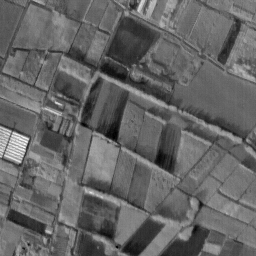
\includegraphics[width=6.4cm,height=6.4cm]{../pan_real.png}};
\coordinate (input-east) at (-3, 0, 0);

\pic[shift={(7,0,0)}] at (input-east) 
    {Ball={
        name =concat_pan,
        fill= \ConcatColor,
        opacity = 0.6,
        radius = 2.5,
        logo= $\pmb{||}$,
        caption= ,
        scale= 1
        }
    };

\draw [connection]  (input-east)    -- node {\midarrow}  (concat_pan-west);

\pic[shift={(0,-2,0)}] at (concat_pan-south) 
    {Ball={
        name =t_pan,
        fill= \PoolColor,
        opacity = 0.6,
        radius = 2.5,
        logo= $\pmb{T}$,
        caption= Pan,
        scale= 1
        }
    };

\draw [connection]  (t_pan-north)    -- node {\midarrow}  (concat_pan-south);
\node[rectangle,
        draw,
dashed,
        ultra thick,
        minimum width = 4cm,
        minimum height = 2cm,        
        label=below:\Huge {}](encoder) at([xshift=10em, yshift=0em]concat_pan-east) {\Huge \textbf{Encoder}};
    
\draw [connection]  (concat_pan-east)    -- node {\midarrow}  (encoder.west);
\node[rectangle,
        draw,
dashed,
        ultra thick,
        minimum width = 4cm,
        minimum height = 2cm,        
        label=below:\Huge {}](bottleneck) at([xshift=10em, yshift=0em]encoder.east) {\Huge \textbf{Bottleneck}};
    
\draw [connection]  (encoder.east)    -- node {\midarrow}  (bottleneck.west);

\pic[shift={(3,0,0)}] at (bottleneck.east) 
    {Ball={
        name =concat_mono,
        fill= \ConcatColor,
        opacity = 0.6,
        radius = 2.5,
        logo= $\pmb{||}$,
        caption= ,
        scale= 1
        }
    };

\draw [connection]  (bottleneck.east)    -- node {\midarrow}  (concat_mono-west);

\pic[shift={(0,-2,0)}] at (concat_mono-south) 
    {Ball={
        name =t_mono,
        fill= \PoolColor,
        opacity = 0.6,
        radius = 2.5,
        logo= $\pmb{T}$,
        caption= Mono,
        scale= 1
        }
    };

\draw [connection]  (t_mono-north)    -- node {\midarrow}  (concat_mono-south);
\node[rectangle,
        draw,
dashed,
        ultra thick,
        minimum width = 4cm,
        minimum height = 2cm,        
        label=below:\Huge {}](decoder) at([xshift=19em, yshift=0em]concat_mono-east) {\Huge \textbf{Decoder}};
    
\draw [connection]  (concat_mono-east)    -- node {\midarrow}  (decoder.west);
\node[rectangle,
        draw,
solid,
        ultra thick,
        minimum width = 6cm,
        minimum height = 4cm,        
        label=below:\Huge {$\mathit{Pan} \rightarrow \hat{T}_\mathit{obj}$}](pan2temp) at([xshift=0em, yshift=-18em]t_pan-south) {\Huge $\sqrt[\leftroot{5} 4]{\frac{\pmb{I_\mathit{pan}} - p^{(0)}_{c_\mathit{pan}}(\pmb{T_\mathit{pan}})}{p^{(1)}_{c_\mathit{pan}}(\pmb{T_\mathit{pan}})}}$};
    \path (input-east) -- (concat_pan-west) coordinate[pos=0.25] (between_in_concat);
            \draw [connection]  (between_in_concat)   --  node {\midarrow} (pan2temp.west-|between_in_concat) --  node {\midarrow} (pan2temp.west);
\draw [connection]  (t_pan-south)    -- node {\midarrow}  (pan2temp.north);
\node[rectangle,
        draw,
solid,
        ultra thick,
        minimum width = 6cm,
        minimum height = 4cm,        
        label=below:\Huge {$\hat{T}_\mathit{obj} \rightarrow Mono$}](temp2mono) at([xshift=0em, yshift=-18em]t_mono-south) {\Huge $p^{(1)}_{c_\mathit{mono}}(\pmb{T_\mathit{mono}}) \pmb{\hat{T}_\mathit{obj}}^4 + p^{(0)}_{c_\mathit{mono}}(\pmb{T_\mathit{mono}})$};
    
\draw [connection]  (pan2temp.east)    -- node {\midarrow} node[above] {\huge $\pmb{\hat{T}_\mathit{obj}}$} (temp2mono.west);

\draw [connection]  (t_mono-south)    -- node {\midarrow}  (temp2mono.north);

\pic[shift={(4,0,0)}] at (temp2mono.east) 
    {Box={
        name=affine,
        caption= ,
        xlabel={{2, }},
        zlabel=256,
        fill = \AffineColor,
        height=32,
        width=1,
        depth=32,
        xlabeloc=0.5,
        }
    };

\draw [connection]  (temp2mono.east)    -- node {\midarrow} node[above] {\huge $\pmb{\hat{I}_\mathit{mono}}$} (affine-west);

\pic[shift={(0,0,0)}] at (decoder.east-|affine-north) 
    {Ball={
        name =pm_sum,
        fill= \SumColor,
        opacity = 0.6,
        radius = 2.5,
        logo= $\pmb{+}$,
        caption= ,
        scale= 1
        }
    };

\draw [connection]  (affine-north)    -- node {\midarrow}  (pm_sum-south);

\draw [connection]  (decoder.east)    -- node {\midarrow}  (pm_sum-west);
\node[rectangle,
        draw,
dashed,
        ultra thick,
        minimum width = 32cm,
        minimum height = 10cm,        
        label=below:\Huge {$\pmb{\tilde{G}_{\mathit{phys}}}$}](phys_model) at([xshift=-8.5em, yshift=-0.75em]temp2mono.center) {\Huge };
    
\pic[shift={ (3.5, 0, 0) }] at (pm_sum-east) 
    {RightBandedBox={
        name=output,
        caption= ,
        xlabel={{1, }},
        zlabel=256,
        fill=\ConvColor,
        bandfill=\ConvReluColor,
        height=32,
        width=0.01,
        depth=32,
        opacity = 0.6,
        bandopacity = 0.6
        }
    };

\node[canvas is zy plane at x=0] (out1) at (output-anchor) {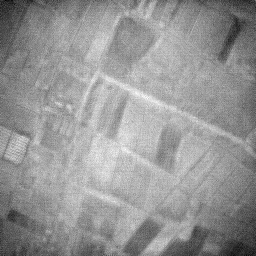
\includegraphics[width=6.4cm,height=6.4cm]{../filt_fake.png}};
\coordinate (out1-east) at (output-anchor);

\draw [connection]  (pm_sum-east)    -- node {\midarrow}  (output-west);

\pic[shift={(-10,-4,0)}] at (phys_model.south) 
    {Ball={
        name =concat,
        fill= \ConcatColor,
        opacity = 0.6,
        radius = 2.5,
        logo= $\pmb{||}$,
        caption= Concatenate,
        scale= 1
        }
    };

\pic[shift={(4,0,0)}] at (concat-east) 
    {Ball={
        name =t_int,
        fill= \PoolColor,
        opacity = 0.6,
        radius = 2.5,
        logo= $\pmb{T}$,
        caption= \\Intrinsic\\Temperature,
        scale= 1
        }
    };

\pic[shift={(4,0,0)}] at (t_int-east) 
    {Ball={
        name =sum,
        fill= \SumColor,
        opacity = 0.6,
        radius = 2.5,
        logo= $\pmb{+}$,
        caption= Summation,
        scale= 1
        }
    };

\pic[shift={(4,0,0)}] at (sum-east) 
    {Box={
        name=affine,
        caption=Affine Transform,
        xlabel={{, }},
        zlabel=,
        fill = \AffineColor,
        height=6,
        width=1,
        depth=6,
        xlabeloc=0.5,
        }
    };
\node[rectangle,
        draw,
solid,
        ultra thick,
        minimum width = 1.5cm,
        minimum height = 1.5cm,        
        label=below:\huge {Calibrated Transform}](calib) at([xshift=15em, yshift=1em]affine-south) {\huge };
    
\end{tikzpicture}
\end{document}
